\section{Preliminaries}

\noindent
\textbf{Blocks and chains.}
The proof-of-work (PoW)~\cite{pow}
blockchain consists of block headers $B = \left<\textsf{ctr}, \textsf{tx}, s\right>$ each of
which contains a \emph{nonce} $\textsf{ctr}$, a short Merkle Tree~\cite{merkle}
root of transaction
data $\textsf{tx}$, and a pointer $s$ to the previous block in the chain~\cite{backbone}. The value $H(B)$, where
$H$ is a hash function modelled as a random oracle~\cite{ro}, is used as the $s'$
to include in the next block. Each block satisfies the PoW equation
$H(B) \leq T$, where $T$ is the \emph{mining target}. In the \emph{static difficulty model}~\cite{backbone,backbone-new},
$T$ is assumed to be a constant (we discuss the variable difficulty model in the appendix).

To address blocks within chain $\chain$, we use $\chain[i]$ to mean the $i^\text{th}$ (zero-based)
block from the beginning and $\chain[-i]$ to mean the $i^\text{th}$ (one-based) block from the end.
$\chain[0]$ indicates \emph{genesis} and $\chain[-1]$ the current tip.
$|\chain|$ denotes the chain length. We use $\chain[i{:}j]$
to denote the subchain starting at the $i^\text{th}$ block (inclusive) and ending at the $j^\text{th}$
block (exclusive).
Omitting $i$ takes the range to the beginning, while
omitting $j$ takes the range to the end.
Similarly, we use $\chain\{A{:}Z\}$ to denote the subchain starting at block $A$
(inclusive) and ending at block $Z$ (exclusive).

Each honest party keeps a local
chain $\chain$, which may be different from the others. It is known~\cite{backbone} these chains
cannot deviate much: The \emph{Common Prefix} property establishes
that they share a long common prefix and only deviate with forks of length up
to a constant $k \in \mathbb{N}$.
Formally, if at any round $r_0$ an honest party $P_0$ has adopted chain $\chain_0$, then
at any round $r_1 > r_0$, any honest party $P_1$ will have adopted a chain $\chain_1$
with $\chain_0[:-k]$ a prefix of $\chain_1$.
This gives rise to ledger \emph{safety}: Any transaction that appears
prior to $C[-k]$ is \emph{confirmed}, and will eventually appear at the same position
in the chains of all honest parties.

The chain of an honest party grows with a certain
rate, which is bounded from below and above with overwhelming probability. This is known as
the \emph{Chain Growth} property (see \cite{backbone} for proof for the
lower bound; a proof of the upper bound is found in the Appendix).
This gives rise to \emph{liveness}: A
transaction submitted to the network will eventually appear confirmed to all honest parties
after at most $\ell \in \mathbb{N}$ blocks. The two security parameters $k$ and $\ell$
that govern the evolution of the chain are polynomial in the underlying cryptographic security parameter
$\kappa$, but constant in the execution time.

\noindent
\textbf{Timelock encryption.}
Timelock encryption allows us to \emph{timelock} a secret so that it can be
unlocked at a prespecified date and time $t$ in the future, but not prior.
It consists of a \emph{timelock}
algorithm $\textsf{timelock}(m, t)$ that takes message $m$ and
timestamp $t$ after which decryption should be possible, and returns ciphertext $c$
encrypted for time $t$, and
 a \emph{timeunlock} algorithm $\textsf{timeunlock}(c, w)$ that takes a
ciphertext $c$ encrypted using $\textsf{timelock}$ and a witness $w$
illustrating that indeed time $t$ has passed, and returns message $m$.
When the time $t$ has elapsed, it becomes easy to compute a \emph{witness} which is
not possible to compute earlier. The
\textsf{timeunlock} function can be called with this witness $w$ for time $t$, and it
returns the original message $m$.
Prior to time $t$, timelock encryption security ensures that
ciphertexts corresponding to the encryptions of two plaintexts $m_1$
and $m_2$ are indistinguishable.

\noindent
\textbf{Witness encryption.}
To construct timelock encryption, we
use \emph{Witness Encryption} (WE)~\cite{timelock-bitcoin}.
In a WE scheme, a plaintext is encrypted into a ciphertext that
can be decrypted \emph{only} if a solution to a computational problem is given.
More concretely, the Witness Encryption scheme is parametrized by
an \textsc{NP} language $\mathcal{L}$ (a decision problem)
and an associated relation $\mathcal{R}$ (which verifies a solution).
For each instance
$x \in \mathcal{L}$, there exists a witness $w$ such that $x\mathcal{R}w$. For
non-instances $x \not\in \mathcal{L}$, no such witness exists. The relation $\mathcal{R}$
is polynomially computable.
A witness encryption scheme consists of an \emph{encryption} algorithm $\textsc{WE.Enc}_\mathcal{R}(m, x)$ that takes plaintext
$m$ and instance $x$ and returns ciphertext $c$ encrypted for this problem instance,
and a \emph{decryption} algorithm $\textsc{WE.Dec}_\mathcal{R}(c, w)$ that takes ciphertext
$c$ and witness $w$ and returns the decrypted plaintext $m$ as long as $x \mathcal{R} w$.
\emph{Correctness} mandates that, whenever $x \mathcal{R} w$, it holds
that $\textsc{WE.Dec}_\mathcal{R}(\textsc{WE.Enc}_\mathcal{R}(m, x), w) = m$.
On the other hand, \emph{security}
mandates that an adversary
given $c = \textsc{WE.Enc}_\mathcal{R}(m, x)$
can extract information about $m$
only if she can also produce
(through a helper \emph{extractor} machine)
a $w$ such that $x \mathcal{R} w$, except with negligible probability.
A correct and secure scheme allows a party to decrypt
\emph{if and only if} she can solve the problem instance by providing a
witness.

To construct timelock encryption using witness encryption, the problem statement asks for the
existence of a series of blockchain work nonces that solve the proof-of-work equation, as illustrated
in Figure~\ref{fig.blockchain-timelock}.
The instantiation of timelock encryption using witness encryption
begins by identifying the chain tip $B$. The timelock time $t$
is expressed in chain time: We ask that a certain number of blocks must have been mined on top of $B$
in order for the secret to become decryptable. The witness encryption \textsc{NP} language contains
the integers $t \in \mathbb{N}$ indicating that there exists a block with additional block height
$t$ descending from the known block $B$. The witness consists of a series of nonces $\textsf{ctr}_i$
and transaction root hashes $\textsf{tx}_i$ such that
$B_0 = B$ and
$B_i = \left<\textsf{ctr}_i, \textsf{tx}_i, H(B_{i-1})\right>$
and $H(B_i) \leq T$,
where $i$ ranges from $1$ to $t$. Therefore, the timelock function $\textsf{timelock}(m, t)$ is defined
as $\textsf{WE.Enc}_\mathcal{R}(m, x)$ where $\mathcal{R}$ corresponds to the relation checking the
validity of the blockchain and $x$ corresponds to the number of blocks $t$ as well as the current
chain tip $B$. The unlock function $\textsf{timeunlock}(c, w)$ is defined as
$\textsf{WE.Dec}_\mathcal{R}(c, w)$ under the same relation $\mathcal{R}$ where $w$ consists of
the sequence of $\textsf{ctr}_i$ and $\textsf{tx}_i$ (c.f., ~\cite{timelock-bitcoin}).

\begin{figure}[ht]
    \caption{Timelock implemented using the moderately hard \textsc{NP} language of chain discovery.
             The problem instance $x = (B, t)$ requests $t = 7$ blocks on top of $B$. The witness
             consists of block headers produced sequentially on top of $B$, irrespective of any
             temporary forks.}
    \centering
    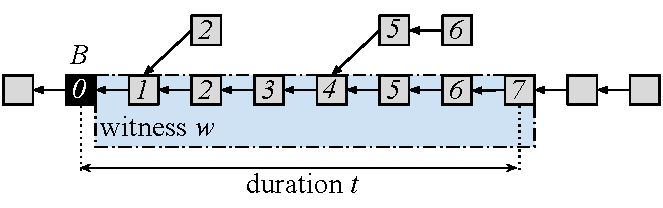
\includegraphics[width=0.55 \columnwidth,keepaspectratio]{figures/blockchain-timelock.pdf}
    \label{fig.blockchain-timelock}
\end{figure}

What is the outcome of encrypting secrets in this manner? Whenever a secret is encrypted
for block time $t$ following block $B$, the secret remains hidden until time $t$ has arrived.
The secret cannot be decrypted prior to that time, because decrypting it would require the decrypting party
to produce (through an extractor) a witness $w$ which is a blockchain of height $t$ extending $B$. However,
due to the \emph{Common Prefix} property of the blockchain, no adversary can do that much sooner than the
honest parties converge to that height (even offline!).
Furthermore, the \emph{chain growth} rate is bounded both \emph{above} 
and \emph{below} by a certain \emph{velocity}, and so, while we do not know its exact growth rate, we can give
an estimate of how quickly it will grow.
With sufficient time elapsed, the miners will produce a witness anyone can use to decrypt the
secret. The result is that no one knows the secret prior to the desired block height, but everyone
knows it afterwards. Because the adversary can have a chain that is leading by up to $k$ blocks, she has
an advantage in decrypting the secret slightly ahead of the honest parties: The
secret begins \emph{leaking} to the adversary at block time $t - k$. This will require us to establish
certain time bounds in our construction.
Our security proof hinges on the \emph{common prefix} property: If
an adversary can decrypt the witness encrypted ciphertext \emph{much} earlier than the honest parties,
she will need to have produced a chain which significantly deviates from the honest parties' chain,
but this is improbable.

Contrary to timelock schemes that require the interested party to devote compute power to decrypt the secret
over time, the scheme using blockchain witnesses allows any party (who can remain offline and have limited compute
power) to take advantage of the scheme.
